% Traceable Decisions Without Backpropagation: Graph Concept Attractors
% for Handwritten Digit Recognition
\documentclass[conference,a4paper]{IEEEtran}

\usepackage[T1]{fontenc}
\usepackage[utf8]{inputenc}
\usepackage{graphicx}
\usepackage{amsmath,amssymb}
\usepackage{booktabs}
\usepackage{multirow}
\usepackage{xcolor}
\usepackage{url}
\usepackage[hidelinks]{hyperref}
\usepackage{fancyhdr}

\newcommand{\cid}[1]{\texttt{#1}}   % concept identifiers: \cid{2\_2}

% DESSERT running header, added to the stock IEEE A4 conference template.
\setlength{\headheight}{28pt}
\pagestyle{fancy}
\fancyhf{}
\renewcommand{\headrulewidth}{0pt}
\fancyhead[C]{\footnotesize\shortstack{%
  The 16th IEEE International Conference on Dependable Systems, Services and Technologies, DESSERT'2026\\
  2--4 October, 2026, Corfu, Greece}}

\begin{document}

\title{Traceable Decisions Without Backpropagation:\\
Graph Concept Attractors for Handwritten Digit Recognition}

\author{
\IEEEauthorblockN{Mykyta Lapin\IEEEauthorrefmark{1},
Kostiantyn Bokhan\IEEEauthorrefmark{1},
Yurii Parzhyn\IEEEauthorrefmark{2},
Kyrylo Perevoznyk\IEEEauthorrefmark{1},
Tetiana Aleksandrova\IEEEauthorrefmark{1}}
\IEEEauthorblockA{\IEEEauthorrefmark{1}Department of Systems Analysis and Information-Analytical Technologies,\\
National Technical University ``Kharkiv Polytechnic Institute'', Kharkiv, Ukraine\\
Mykyta.Lapin@cit.khpi.edu.ua, kostiantyn.bokhan@khpi.edu.ua,\\
kyrylo.perevoznyk@cs.khpi.edu.ua, Tetiana.Aleksandrova@khpi.edu.ua}
\IEEEauthorblockA{\IEEEauthorrefmark{2}School of Computer and Cyber Sciences, Augusta University, Augusta, GA, USA\\
yparzhyn@augusta.edu}
}
% ORCID (verified, see project canonical table):
%   Lapin        0009-0003-6307-1172
%   Bokhan       0000-0003-3375-2527
%   Parzhyn      0000-0001-5727-1918
%   Perevoznyk   0009-0009-2327-1501
%   Aleksandrova 0000-0001-9596-0669

\maketitle
\thispagestyle{fancy}

\begin{abstract}
Post-hoc explanation methods approximate a trained model from the outside, and a model can be built so that the explanation hides the behaviour it is meant to expose. We build a recogniser whose decision is already an inspectable object. Each grey-scale image is converted into an attributed bipartite graph: Point nodes mark the endpoints, corners and intersections of the contour skeleton, and Vector nodes mark the straight segments between them. For every class we form a concept attractor by structural reduction, merging training graphs one at a time and generalizing attribute values to intervals. No gradient is computed and no backpropagation is used. A test image is classified by graph edit distance against every concept attractor, with a winner-take-all rule. We evaluate on the MNIST test images whose contours are complete: the completeness filter admits 8,707 of 10,000, and every reported metric is conditional on it. Thirteen concept attractors formed from 76 unique training samples (805 images after augmentation) classify 8,685 images with 91.13\% accuracy, 91.92\% precision, 91.13\% recall and 91.34\% F1 score. We trace one decision from the input image through the winning concept attractor down to the per-feature costs, and we report inference cost measured per pipeline stage; the classification stage has a median of 167 ms on a profiled subset of 770 misclassified images, which is not a typical-case estimate. We report a research prototype and make no comparison with neural classifiers.
\end{abstract}

\begin{IEEEkeywords}
explainable artificial intelligence, graph-based image representation, concept attractor, structural reduction, graph edit distance, traceable decision
\end{IEEEkeywords}

\section{Introduction}

Recognition systems reach high accuracy and return a label without showing the evidence behind it. Where a decision has to be justified to an operator, a clinician or an auditor, that opacity is a separate problem from how often the model is correct.

The usual remedy is a post-hoc explanation. LIME builds a local linear approximation of a trained model around one example \cite{ribeiro2016}. SHAP distributes feature contributions using a cooperative-game scheme \cite{lundberg2017}. Both work from outside the model and treat it as a black box, so the explanation describes a surrogate function. Slack et al.\ showed that the gap can be exploited: a classifier with an explicit bias can be built so that LIME and SHAP hide that bias \cite{slack2020}. Rudin argues that high-stakes decisions call for a model interpretable by construction \cite{rudin2019}. We take that position.

In our system the structure of the representation carries the explanation. The contour of an image is encoded as an attributed graph whose nodes are characteristic points and the segments between them, with geometric and semantic attributes stored on the nodes themselves. A cycle in the graph corresponds to a closed contour, node degree describes branching, and an attribute interval states how far that feature may vary inside a class. We build no explanation module on top of the classifier.

The system is a prototype built for research. It does not claim the accuracy of neural classifiers on benchmark data and we do not compare it against them. Our question is whether recognition is possible without backpropagation, from a small number of training samples, with a decision path a reader can follow from end to end.

The paper contributes: (i) a graph representation and a concept formation procedure that use no gradient and no backpropagation; (ii) an evaluation on MNIST under a completeness filter we state in full, with its per-class skew; (iii) a worked decision trace that explains one correct decision and the dominant error; and (iv) inference cost measured per pipeline stage on run artefacts.

\section{Related Work}

Baniecki and Biecek survey attacks on explanations: explanations can be manipulated, fooled or fairwashed, and the survey catalogues the resulting insecurities \cite{baniecki2024}. The alternative design direction is a model interpretable by construction \cite{rudin2019}. Forest et al.\ apply concept bottleneck models to prognostics, taking degradation modes as the intermediate concepts so a prediction decomposes per component \cite{forest2025}; the mapping from input to concept is still a trained network. Garc\'ia-Cuesta et al.\ show that the prototypes of prototype-based networks can be altered while the explanation keeps its plausibility \cite{garciacuesta2025}. Interpretability by construction therefore needs representation elements with a geometric meaning outside any learned embedding space.

Structural representations of shape are long established. Vision GNN treats an image as a graph of patch nodes and runs message passing over it \cite{han2022}. Chatbri et al.\ compare contours and skeletons for matching binary images \cite{chatbri2016}; Shen et al.\ combine the two, recognising shapes from a bag of skeleton-associated contour parts \cite{shen2016}. Gan et al.\ represent handwritten Chinese characters by skeleton graphs and run a graph transformer over them \cite{gan2023}; by choice of representation this is the closest prior work to ours. There the network weights determine the decision; here the image graph is matched against a concept attractor and the answer is a list of node substitutions with their costs.

Conte et al.\ survey thirty years of exact and approximate graph matching \cite{conte2004}. Graph edit distance (GED) gives a dissimilarity that decomposes into elementary operations on nodes and edges. Riesen and Bunke approximate GED by bipartite assignment, which made it usable at practical graph sizes \cite{riesen2009}. Wang et al.\ learn the A* search heuristic for GED and recover the edit path \cite{wang2021}, and Piao et al.\ recover the edit path from a predicted matching matrix, noting that models which reduce GED to similarity regression produce no operation sequence \cite{piao2023}. In formulations that regress similarity directly, an elementary operation has no predefined cost, so a single cost term does not say which feature separates two matched nodes.

Work on alternatives to backpropagation continues. The Forward-Forward algorithm replaces the backward pass with two forward passes and a local objective \cite{hinton2022}, and a survey of neuro-symbolic integration describes systems in which an explicit symbolic part carries explainability and formal reasoning \cite{nawaz2025}. Few-shot learning is dominated by meta-learning: prototypical networks build a class prototype as a centroid in a learned embedding space \cite{snell2017}, MAML learns initial weights that a few gradient steps adapt to a new task \cite{finn2017}, and Lake et al.\ learn a character from one example with a generative program model \cite{lake2015}. We cite these as context for the problem setting and make no accuracy comparison against them. The paper continues our own graph model of few-shot learning without backpropagation \cite{lapin2025fewshot} and the information-architecture frame behind it \cite{parzhyn2025architecture}.

The reviewed work leaves three conditions unmet at once. The structure of the representation should carry both the decision and the explanation. Matching costs should be tied to predefined geometric properties instead of being learned from data. The result should come from tens of training samples without backpropagation. This paper addresses that combination.

\section{Method}

\subsection{Graph Representation}

We represent a digit image by an attributed bipartite graph whose two kinds of node alternate: a Point node is a characteristic point of the contour, a Vector node the straight segment between two neighbouring points. Links are bidirectional, so every traversal has the form Point $\rightarrow$ Vector $\rightarrow$ Point; no two Point nodes are joined directly. Pixel values are not used after the graph is built. Making a segment a node rather than an edge gives it attributes of its own --- length, direction, orientation --- so it takes part in comparison like a point.

Point nodes have four types: an EndPoint terminates an open contour, a CornerPoint marks a sharp change of direction and stores the angle, an IntersectionPoint marks a crossing of lines, and a StartPoint fixes where traversal begins. One node can carry several of these labels at once.

A Point node stores its $x$ and $y$ coordinates and their normalized values. A Vector node stores both endpoints, the length, the quadrant (I--IV, or $-1$ for an axis-aligned segment), the horizontal direction (LEFT, RIGHT, NONE) and the vertical direction (TOP, BOTTOM, NONE); quadrant and directions describe orientation without absolute coordinates. Coordinates are normalized to a centred range from $-1$ to $1$ by~\eqref{eq:norm}:
\begin{equation}\label{eq:norm}
x_{norm} = \frac{x - c_x}{\rho}, \qquad y_{norm} = \frac{y - c_y}{\rho}
\end{equation}
where $(c_x, c_y)$ is the centre of the bounding box of the graph's points and $\rho = \sqrt{h_w^2 + h_h^2}$ its half-diagonal, built from the half-width $h_w$ and the half-height $h_h$; the denominator is the same for both axes and values are rounded to one decimal. Because the centre and the scale come from the graph's own bounding box, the normalized coordinates do not depend on where the digit sits in the image or how large it is drawn.

\subsection{Image-to-Graph Pipeline}

\begin{figure*}[t]
\centering
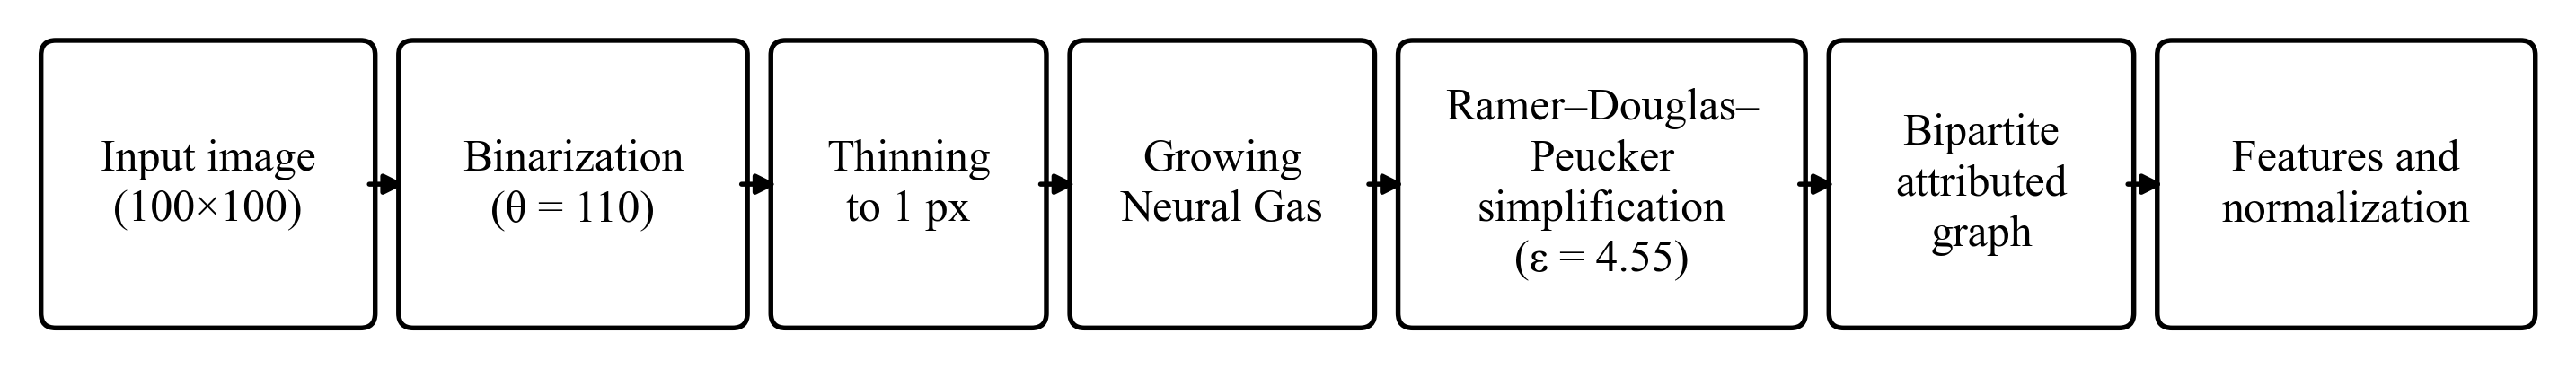
\includegraphics[width=\textwidth]{figures/fig_pipeline.png}
\caption{The six stages that turn a $100 \times 100$ grey-scale image into an attributed bipartite graph: binarization at $\theta = 110$, thinning to one pixel, growing neural gas, Ramer--Douglas--Peucker simplification at $\varepsilon = 4.55$, construction of the Point and Vector nodes, and attribute extraction with coordinate normalization.}
\label{fig:pipeline}
\end{figure*}

MNIST images are grey-scale and are upscaled from $28 \times 28$ to $100 \times 100$ pixels by Lanczos resampling. The graph is built in six stages (Fig.~\ref{fig:pipeline}). The image is binarized at $\theta = 110$. The binary mask is cleaned by small-object removal and morphological closing, then thinned to one-pixel width by the Zhang--Suen algorithm \cite{zhang1984}; skeleton branches shorter than 8\% of the total skeleton length are pruned. The skeleton is approximated by a growing neural gas \cite{fritzke1995}, whose network of nodes reproduces the topology of the skeleton lines. That network is simplified by the Ramer--Douglas--Peucker algorithm with $\varepsilon = 4.55$ \cite{douglas1973}, which drops nodes lying almost on a straight line. The bipartite graph of Point and Vector nodes is built on the simplified network, and the last stage computes node attributes and normalizes coordinates.

$\theta = 110$ is the starting threshold of a retry ladder: if the resulting skeleton graph is disconnected, the pipeline re-runs at $\theta - 5$, down to 20; only $\varepsilon = 4.55$ is fixed. The same pipeline runs on training images during concept formation and on test images during classification.

\subsection{Concept Formation by Structural Reduction}

A concept attractor is formed iteratively, one training sample at a time. Its initial value is the graph of the first sample, $C_0 = G_1$, and each further sample refines it by a custom reduction operation (CRO), \eqref{eq:cro}:
\begin{equation}\label{eq:cro}
C_{i+1} = \mathrm{CRO}(C_i,\, G_{i+1}), \quad i = 1, \ldots, n-1
\end{equation}
where $C_i$ is the current state, $G_{i+1}$ the graph of the next sample and $n$ the number of samples. Processing one sample aligns the start points, applies the reduction strategies to critical points, traverses both graphs synchronously, and merges the properties of corresponding nodes. The synchronous traversal finds a maximum common minor of the two graphs, so a stroke of three nodes in one sample can match five in another. The reduction leaves the structure that repeats in every sample of the class.

Three reduction strategies are applied. Endpoint removal deletes an EndPoint with no counterpart in the second graph, together with the path from it to the nearest critical point. Intersection merging reclassifies an IntersectionPoint of degree at most two as a CornerPoint or an EndPoint and deletes surplus intersections, least similar first. Corner-point reduction matches sub-paths between non-corner critical points and removes surplus CornerPoints from the longer path, lowest similarity first. The intersection strategy demotes a node from IntersectionPoint to CornerPoint to Point. At inference a concept node matches an image node only if the concept node's labels are a subset of the image node's labels, so a concept attractor is never more specific than the images it matches. StartPoint is never reduced; it fixes the entry point of traversal.

Attributes are generalized with the structure. A numeric attribute becomes an interval with three values: minimum, maximum and centre. A categorical attribute survives only if it agrees across all samples, and label lists are replaced by their intersection.

The procedure consumes every sample it is given, in a fixed order by image identifier. The number of samples per concept attractor was chosen during authoring by one criterion: further samples no longer changed the concept attractor. The procedure follows the energy model of concept formation in our earlier work \cite{parzhyn2025energy}; its invariant formulation, with concept formation as hypergraph attractor dynamics, is in \cite{lapin2026invariant}.

\subsection{Training Data and Sample-Selection Policy}

The alphabet holds 13 concept attractors for 10 digit classes. Classes 1, 2 and 4 have two each --- \cid{1\_1} and \cid{1\_3}, \cid{2\_1} and \cid{2\_2}, \cid{4\_1} and \cid{4\_2} --- because these digits are written in two topologically different styles that no reduction turns into one another; the other seven classes have one each. Sizes run from 3 to 12 nodes: the largest is \cid{2\_2} with 12, the smallest \cid{1\_3} with 3; the single concept attractor of digit 7, \cid{7\_1}, has 5.

The 13 concept attractors were formed from 76 unique MNIST \cite{lecun1998} training samples, 3 to 9 each. The count per concept attractor follows from the criterion in Section III-C; no quota was fixed in advance. Each sample carries about ten augmented variants --- a small random rotation and translation --- giving 805 training images.

We chose the samples by hand. They are not a random draw from the training split; the criterion was the least distorted writings, with no gaps in the contour. The choice rests on an assumption: an instance of a class that a person reads correctly already carries all the structural and topological features of that class. Formation then needs a small number of structurally complete writings rather than a representative sample of the distribution. Variation enters through augmentation --- the chosen samples fix the structure, and their augmented variants set the bounds of the parameter intervals.

The limits of this assumption are only partly known: we did not measure how sensitive accuracy is to the specific choice of samples, so we cannot say how much a different selection would change the result.

\subsection{Classification by Graph Edit Distance}

Classification matches the image graph against every concept attractor in the alphabet. A complexity pre-filter runs first: the complexity of a graph is $\kappa = |V| + |E|$, and concept attractors more complex than the image graph are dropped before any distance is computed.

GED is the minimum total cost of the insertions, deletions and substitutions of nodes and edges that turn one graph into another. Exact GED is NP-hard, so practical systems approximate it \cite{riesen2009}. We use an anytime solver with a deadline of 5 s per comparison, which returns the best edit path found by then. Substitution costs follow a monotone ladder: NO\_COST $= 0$, MINOR $= 0.25$, GENERAL $= 0.5$, SEVERE $= 0.8$, NO\_MATCH $= 1.0$ and IMPOSSIBLE $= 6.0$. IMPOSSIBLE is assigned to incompatible node types; its cost blocks the substitution in practice. Inserting a node costs IMPOSSIBLE, so a concept attractor node without an image counterpart blocks the match; deleting a node costs MINOR. Deleting an edge costs MINOR, inserting one NO\_COST, and edges themselves are not compared.

Node comparison uses 13 features: normalized $x$, normalized $y$, distance to centroid, horizontal direction, vertical direction, angle with the $x$ axis, minimum junction angle, endpoint indicator, corner indicator, length ratio to maximum, average neighbouring vector length, neighbouring endpoint count and neighbouring junction count. Nine of them store an interval in the concept attractor node and take a diagnostic weight, \eqref{eq:weight}:
\begin{equation}\label{eq:weight}
w_f = \frac{s_f}{\Delta_f + \varepsilon_w}
\end{equation}
where $\Delta_f$ is the interval width, $\varepsilon_w = 0.1$ smooths the denominator and $s_f = 1$. A narrow interval means the feature was stable across the training samples, so it weighs more; a wide interval barely affects the cost. The other four features are categorical and have no interval: the two directions take $s_f = 0.6$, the endpoint and corner indicators $0.4$. Weights are normalised over the features present on both nodes, $\tilde w_f = w_f / \sum_g w_g$. A value inside the interval costs $\tilde w_f\,|v - c_f| / (\Delta_f / 2)$, zero at the centre $c_f$ and $\tilde w_f$ at the edge. A value outside costs the full NO\_MATCH penalty of 1.0, unweighted. A node's substitution cost is the sum over its features, so one out-of-range feature alone lifts it above 1.0.

The total edit cost $c$ becomes a similarity by~\eqref{eq:sim}:
\begin{equation}\label{eq:sim}
\mathrm{sim}(G_1, G_2) = 1 - \frac{c}{c + \max(\kappa_1,\, \kappa_2)}
\end{equation}
where $\kappa_1$ and $\kappa_2$ are the complexities of the two graphs. Similarity lies between 0 and 1; normalizing by the larger graph keeps it comparable across concept attractors of different size. Selection is winner-take-all on a score corrected for complexity, \eqref{eq:score}:
\begin{equation}\label{eq:score}
\mathrm{score} = \mathrm{sim} + \lambda \log_2 \kappa
\end{equation}
with $\lambda = 0.10$, a mild preference for more complex concept attractors when similarities are close. The highest score among the concept attractors that passed the pre-filter wins. If none activates, the image is marked unrecognized.

\section{Results}

\subsection{Evaluation Data and the Completeness Filter}

We evaluate on the MNIST test set \cite{lecun1998}, 10,000 handwritten digit
images rendered at 100$\times$100 pixels. The completeness filter is a per-image
annotation made by hand before any classification run and recorded in
\texttt{mnist\_all\_manifest.csv} in the public repository: an image is marked
complete when its stroke has no break and incomplete otherwise. The annotation
uses only that structural property, not the class label and not the
classifier's output. A broken stroke
violates the assumption the graph representation of Section~III rests on, and
the graph built from such an image describes a different figure. Recognising
broken structures needs a separate mechanism, associative recognition, which
the system does not implement.

The filter admits 8,707 of the 10,000 test images and excludes 1,293, or
12.9\%. The accuracy reported below is therefore conditional on the filter
and does not transfer to full MNIST. The filter also acts unevenly across
classes (Table~\ref{tab:perclass}). Class~1 keeps 1,129 of its 1,135 test
images (99.5\%), while class~8 keeps 582 of 974 (59.8\%). Per-class figures
therefore rest on samples of very different size, and class~8 has the narrowest
basis.

A further 22 admitted images (0.25\%) failed graph construction:
skeletonization produced no connected graph at any threshold of the retry
ladder (Section III-B). We count these as pipeline
errors. A classification decision was produced for 8,685 images.

\subsection{Classification Results}

On the 8,685 classified images the system reaches 91.13\% accuracy,
91.92\% precision, 91.13\% recall and 91.34\% F1. The three averaged
figures are weighted by class support; the unweighted macro averages over the
ten classes are 92.22\%, 91.22\% and 91.54\%.

\begin{table}[t]
\caption{Per-class evaluation. ``Admitted'' is the count passing the
completeness filter and ``share'' its fraction of that class in the MNIST test
set. ``Classified'' is the count that produced a classification decision;
precision, recall and F1 are computed on that column and the totals are
support-weighted.}
\label{tab:perclass}
\centering
\footnotesize
\setlength{\tabcolsep}{3pt}
\begin{tabular}{lrrrrrr}
\toprule
Class & Admitted & Classified & Share, \% & Prec., \% & Recall, \% & F1, \% \\
\midrule
0     & 830   & 830   & 84.7 & 99.87 & 91.93 & 95.73 \\
1     & 1,129 & 1,122 & 99.5 & 93.69 & 96.52 & 95.08 \\
2     & 956   & 955   & 92.6 & 92.28 & 77.59 & 84.30 \\
3     & 969   & 968   & 95.9 & 91.78 & 95.76 & 93.73 \\
4     & 953   & 950   & 97.0 & 92.15 & 84.00 & 87.89 \\
5     & 796   & 796   & 89.2 & 93.97 & 91.96 & 92.95 \\
6     & 742   & 741   & 77.5 & 84.88 & 92.44 & 88.50 \\
7     & 1,014 & 1,011 & 98.6 & 82.01 & 95.15 & 88.10 \\
8     & 582   & 581   & 59.8 & 98.74 & 94.49 & 96.57 \\
9     & 736   & 731   & 72.9 & 92.85 & 92.34 & 92.59 \\
\midrule
Total & 8,707 & 8,685 & 87.1 & 91.92 & 91.13 & 91.34 \\
\bottomrule
\end{tabular}
\end{table}

Per-class figures spread much wider than the totals
(Table~\ref{tab:perclass}). Precision is highest for class~0 (99.87\%) and
class~8 (98.74\%), whose concepts attract almost nothing from other classes.
Precision is lowest for class~7 (82.01\%) and class~6 (84.88\%), which take
on images belonging to neighbouring classes. Recall orders the classes
differently, with class~2 (77.59\%) and class~4 (84.00\%) at the bottom.

The system made 770 wrong decisions: 726 assigned the image to a wrong class,
and in 44 no concept activated and the image was left unrecognised, mostly in
class~6 (16) and class~8 (14).

\begin{figure}[t]
\centering
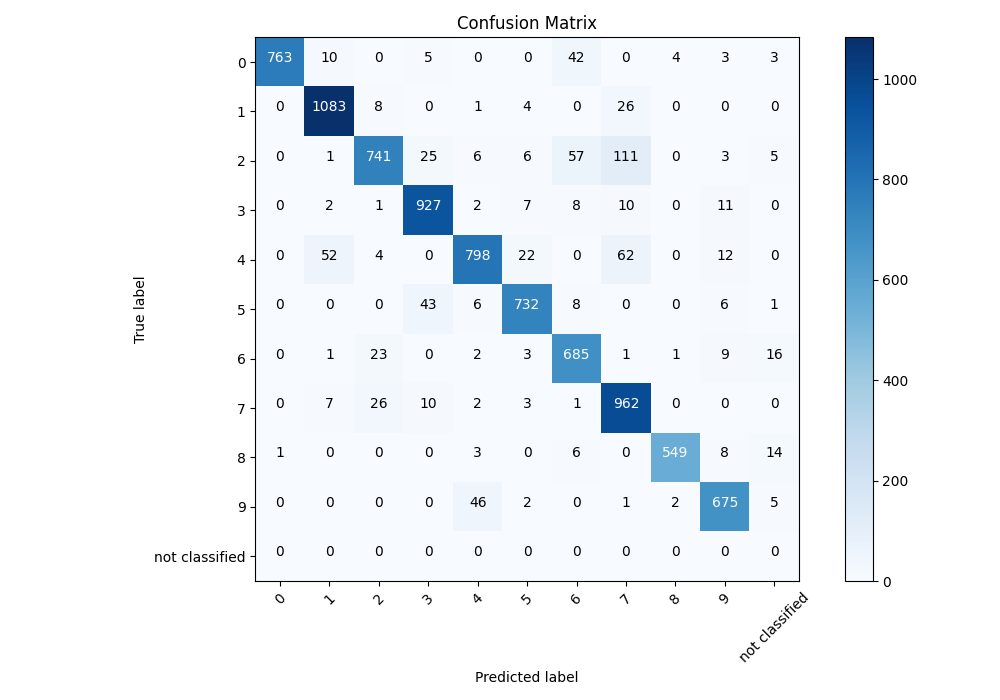
\includegraphics[width=\columnwidth,trim=96 13 60 27,clip]{figures/fig_confusion.png}
\caption{Confusion matrix over the 8,685 classified images, taken from the run
artefacts. Rows are true classes, columns predicted classes; the last column
holds images that activated no concept, and the last row is empty by
construction.}
\label{fig:confusion}
\end{figure}

Errors concentrate on a few pairs (Fig.~\ref{fig:confusion}). Written as true
class $\rightarrow$ predicted class, the most frequent pairs are
2$\rightarrow$7 with 111 cases, 4$\rightarrow$7 with 62, 2$\rightarrow$6 with
57, 4$\rightarrow$1 with 52, 9$\rightarrow$4 with 46, 5$\rightarrow$3 with 43,
0$\rightarrow$6 with 42, 1$\rightarrow$7 with 26, 7$\rightarrow$2 with 26, and
2$\rightarrow$3 with 25. These ten pairs cover 490 of the 726 wrong-class
assignments, or 67.5\%. Two classes produce nearly half of all errors:
class~2 with 214 and class~4 with 152.

\subsection{Decision Trace}

Every decision decomposes into values a reader can check. We show this on
image \cid{mnist\_test\_2\_00766}, true class 2, predicted 7. We chose a
misclassification: an explanation has to hold for a wrong decision as well
as for a correct one. Fig.~\ref{fig:trace} shows the construction of the graph and the two
competing concepts; Table~\ref{tab:trace} gives the decision trace.

\begin{figure*}[t]
\centering
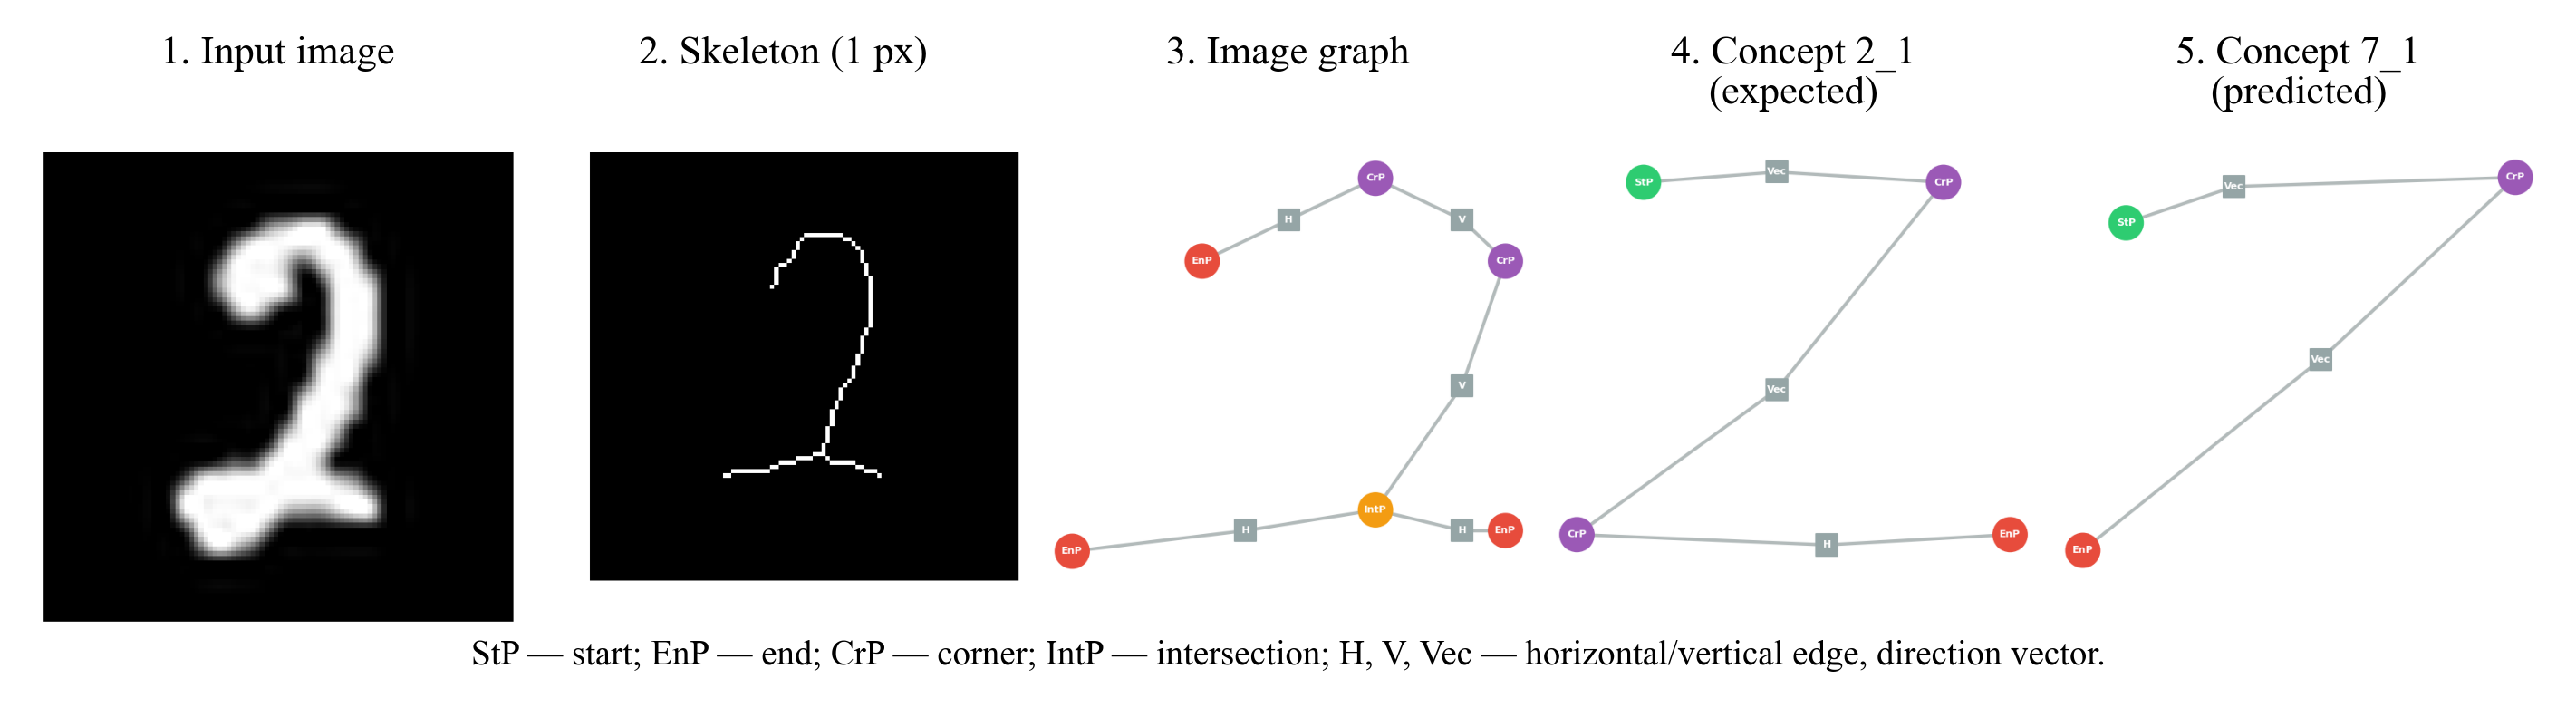
\includegraphics[width=\textwidth]{figures/fig_trace.png}
\caption{Decision trace for \cid{mnist\_test\_2\_00766}, in five panels: the
input image; the 1-pixel skeleton; the image graph with Point and Vector nodes;
concept \cid{2\_1}, expected; concept \cid{7\_1}, predicted. The lower loop of
the digit is already absent in the skeleton, so the image graph carries neither
a cycle nor an intersection point.}
\label{fig:trace}
\end{figure*}

The image graph has complexity 21. The complexity pre-filter runs first. The
richer concept of digit~2, \cid{2\_2}, has 12 nodes and complexity 24, so the
condition $24 > 21$ removes it before any comparison. The impoverished input is
visible in the image: binarization lost the lower loop of the 2, the closed
structure became an open spur, and the graph holds neither a cycle nor an
intersection point.

Two concepts then compete. Concept \cid{7\_1} has five nodes, every one of them
substituted within the learned intervals of the concept, at substitution costs
between 0.04 and 0.39, and reaches similarity 0.8317. Concept \cid{2\_1} has
seven nodes and matches the input structurally, but three of its nodes each
carry one feature outside its interval, and each takes the full 1.0 penalty:
the StartPoint on \texttt{distance\_to\_centroid} (0.56 against $[0.69, 1.00]$),
a CornerPoint on \texttt{normalized\_x} (0.20 against $[-0.70, 0.10]$) and a
horizontal Vector node on \texttt{length\_ratio\_to\_max} (0.31 against
$[0.43, 1.00]$). With their in-range features added, the three node
substitution costs are 1.01, 1.10 and 1.30. Its similarity is 0.7300.

Complexity is $\kappa = 9$ for \cid{7\_1} and $\kappa = 13$ for \cid{2\_1}, so
the prior of \eqref{eq:score} favours \cid{2\_1} by 0.053 and does not close
the gap. Winner-take-all on the score picks \cid{7\_1}: 1.149 against 1.100.

\begin{table}[t]
\caption{Decision trace for \cid{mnist\_test\_2\_00766}.}
\label{tab:trace}
\centering
\footnotesize
\setlength{\tabcolsep}{3pt}
\begin{tabular}{lrrp{3.0cm}rr}
\toprule
Concept & Nodes & $\kappa$ & Matching outcome & Sim. & Score \\
\midrule
\cid{2\_2} & 12 & 24 & removed by the pre-filter, $24 > 21$ & --- & --- \\
\cid{7\_1} & 5 & 9 & all five nodes substituted inside the intervals, costs
0.04--0.39 & 0.8317 & 1.149 \\
\cid{2\_1} & 7 & 13 & three nodes with one out-of-range feature each; node costs
1.01 / 1.10 / 1.30 & 0.7300 & 1.100 \\
\bottomrule
\end{tabular}
\end{table}

The mechanism holds beyond this one image. Across all 111 2$\rightarrow$7
errors, \cid{2\_1} entered the comparison every time and lost on similarity
every time, by a mean margin of 0.14. In none of the 111 cases did a concept of
digit~2 win on similarity and then lose after the complexity prior was applied.

\subsection{Inference Cost}

An image is compared against at most 13 concepts, each comparison under a
5\,s deadline, so the theoretical upper bound is 65\,s per image. The measured
stage times stay far below it.

The pipeline ran on a single workstation in 24 Docker containers: four
skeletonization instances, four contour analysis instances and sixteen
classification instances. Per-stage medians come from the profiling records:
skeletonization 52.8\,ms with a maximum of 533\,ms, contour analysis
211.5\,ms with a maximum of 1,905\,ms, and the classification stage, meaning
all GED comparisons for one image together, 167.1\,ms with a 99th percentile of
about 0.84\,s and a maximum of 1,414\,ms. No profiled image came close to the
5\,s deadline of a single comparison. On the profiled images the solver
therefore finished its search before the deadline, and the reported distances
are completed results, not deadline-truncated ones.

One caveat limits the use of these medians. Profiling records exist only for
the 770 misclassified images, so the profiled subset is biased and
correctly classified images are absent from it. The available data does not fix
the direction of the bias. The number of GED comparisons per image is set by
the complexity pre-filter, not by the correctness of the final decision. The medians are therefore not a typical-case estimate.
The run does not record its own total duration, and the system does not store
the time of an individual GED comparison.

\section{Discussion}

The explanation here is the decision object itself. No second model
approximates the classifier from outside. To see why an image received a class,
a reader opens the image graph and reads the learned intervals of the winning
concept attractor and the cost charged for each feature. The trace in
Section~IV-C runs the whole chain, from the complexity pre-filter down to one
out-of-range value, \texttt{normalized\_x} at 0.20 against the interval
$[-0.70, 0.10]$. Post-hoc attribution methods build
their explanation after the fact by perturbing the input
\cite{ribeiro2016,lundberg2017}, and that construction can be manipulated
\cite{slack2020}. Decisions with consequences are better taken by models
interpretable by construction \cite{rudin2019}.

The same property applies to the failures. Binarization loses the lower loop of
the digit, so the image graph carries no intersection point, and the pre-filter
removes \cid{2\_2} in 86 of the 111 2$\rightarrow$7 cases. The pre-filter is
not the cause: in a control run with it lifted, \cid{2\_2} won none of the 111,
because an intersection-point condition blocks its match to a graph without an
intersection. The error has two causes: the lower loop lost at binarization,
and the full interval penalties on \cid{2\_1} against the in-interval match of
the five-node \cid{7\_1}. The error can be named and its prevalence checked
over all 111 cases.

Traceability defines the application niche: tasks where the answer has to be
auditable. Verification of handwritten marks in document workflows, inspection
of industrial marking, and tutoring systems that must show a learner the reason
for a grade share the property that a human resolves every disputed decision. A
decision record of the named concept, its node substitutions and its
per-feature costs goes into that review without a separate explanation module.
For a dependability audience the property on offer is auditability: every
decision leaves a record that a person can check against the input without
re-running the system.
The small training set also lowers the cost of starting on a new set of marks:
one concept attractor forms from 3--9 samples and their augmented variants
(Section III-D). An earlier
prototype reported 82.44\% on six classes \cite{parzhyn2025energy}; the two
numbers are not comparable, since the class set, the test set size and the
formation procedure all differ.

Several limitations bound the result. The headline metric is conditional on the
completeness filter, which excludes 12.9\% of the test set unevenly across
classes. The inference cost is measured, but the profiled subset holds only
misclassified images, and per-comparison timing does not exist. The 76 training
samples were selected by hand and the sensitivity of accuracy to that selection
was not measured, so part of the accuracy may come from a fortunate choice. The
training samples were chosen on the same completeness criterion as the test
filter, so the evaluation measures the system inside the regime it was built
for, and the exclusion does the most work in the classes with the lowest
admission rates (8, 9 and 6). Sensitivity of a concept attractor to the
order of its samples was not measured in this study. Tolerance to rotation is
limited to the small range covered by augmentation. The contour representation
discards texture and gradients, which confines the method to silhouette and
stroke images. Broken contours need associative
recognition, which the system does not have.

\section{Conclusion}

We formed an alphabet of 13 concept attractors for ten digit classes by
structural reduction of 76 hand-selected training samples and their augmented
variants, with no backpropagation anywhere in the procedure. Classification by graph edit
distance with interval-based feature weighting recognises 8,685
complete-contour MNIST images at 91.13\% accuracy, 91.92\% precision,
91.13\% recall and 91.34\% F1. The evaluation is stated with its filter:
12.9\% of the test set is excluded and the metric does not carry over to
full MNIST. Each decision decomposes into a named concept, a list of
node substitutions and a per-feature cost, and the dominant 2$\rightarrow$7
error was traced through that decomposition over all 111 cases. Inference cost
was measured per pipeline stage, and on the profiled images the 5\,s deadline of a
single comparison was not reached. Work ahead covers associative recognition for broken
contours, per-comparison timing on the full test set, and a sensitivity study
of the training sample choice. The source code and the run artefacts are public
at \url{https://github.com/kbokh/NaturalAGI}.


\bibliographystyle{IEEEtran}
\bibliography{references}

\end{document}
